\graphicspath{{chapters/chapter4/imgs/}}

\chapter{Planowany eksperyment}\label{chapter:ch4}

W tej sekcji przedstawiony zostanie pełny plan eksperymentu, w tym: projekt gry przeglądarkowej
z gatunku \textit{visual novel}, opis implementacji i wykorzystania generatywnych agentów
opartych na dużych modelach językowych oraz sam przebieg badań.

\section{Projekt gry wykorzystanej w eksperymencie}\label{section:ch4_1}

Celem gry ma być oczywiście zbadanie wpływu wykorzystania generatywnych agentów na zaangażowanie
grającego w narrację. W związku z tym rozgrywka powinna kłaść nacisk przede wszystkim na
przedstawianie treści fabularnych, pozostawiając walory estetyczne czy mechaniki gry na drugim
planie. Dodatkowo, całe doświadczenie powinno mieścić się w przedziale 15-30min i być dostępne
w łatwy sposób (bez instalacji). Z uwagi na te założenia zdecydowano się na utworzenie gry
dwuwymiarowej z gatunku \textit{visual novel} (Patrz sekcja poniżej).

\subsubsection*{Gatunek \textit{visual novel}}\label{subsubsection:ch4_1_1}

Forma \textit{visual novel} (z ang. \textit{powieść wizualna}) jest najczęściej uznawana jako
gatunek gier komputerowych, choć niektórzy dostrzegają w niej zupełnie odrębne od gier
medium\cite{tvtropes_visual_novel}.

Kluczowymi cechami \textit{visual novel} są prezentacja tekstu za pomocą okienek dialogowych, które gracz
musi klikać, aby przejść dalej, oraz statyczne grafiki przedstawiające postacie i otoczenie. Choć
powieści wizualne często zawierają elementy multimedialne, takie jak animacje, muzyka czy dubbing,
to nie są one ich kluczowymi składnikami\cite{tvtropes_visual_novel}.

\textit{Visual novel} koncentrują się przede wszystkim na prezentacji narracji, z niewielką lub zerową
ilością rozgrywki. Wiele z nich oferuje nieliniową, rozgałęziającą się fabułę z wieloma
zakończeniami i systemem wyborów wpływających na dalszy przebieg wydarzeń\cite{tvtropes_visual_novel}.
Z drugiej strony, istnieją też powieści wizualne
pozbawione jakiejkolwiek rozgrywki i rozgałęzień fabularnych, określane mianem
\textit{kinetic novel}\cite{tvtropes_kinetic_novel}.

Ogólnie powieści wizualne wyróżniają się dominacją narracji przedstawianej za pomocą tekstu i grafik nad
rozgrywką. Kryterium odróżniające je od gier przygodowych jest stopień, w jakim faktycznie
wykorzystują mechaniki gry i gameplay w stosunku do narracji\cite{tvtropes_visual_novel}.

\subsubsection*{Projekt gry}

Gra została opracowana przy wykorzystaniu silnika Ren'Py w wersji 8.2.1, opartego na języku Python.
Ren'Py to popularne narzędzie służące do tworzenia gier tego rodzaju, oferujące zaawansowane
możliwości pisania scenariuszy, zarządzania obrazami i dźwiękiem oraz tworzenia systemów wyborów
i rozgałęzień fabularnych.

Wszystkie niezbędne zasoby graficzne pozyskane zostały ze społeczności twórców niezależnych na
platformie itch.io. Grafiki postaci i tła zostały wyprodukowane przez twórców
LinXueLian (\url{https://linxuelian.itch.io/}) oraz Potat0Master (\url{https://potat0master.itch.io/}),
specjalizujących się w tego typu materiałach na potrzeby \textit{visual novel} i gier przygodowych.

Po zakończeniu prac, gotowy produkt został wyeksportowany do postaci pliku wykonywalnego
kompatybilnego z przeglądarkami internetowymi. Takie rozwiązanie umożliwia graczom pobieranie i
uruchamianie tytułu bezpośrednio ze stron www, bez konieczności instalowania dodatkowego
oprogramowania.

Finalną wersję gry opublikowano na platformie dystrybucji cyfrowej itch.io, która stała się
głównym kanałem udostępniania produkcji odbiorcom. Itch.io jest popularnym hubem dla niezależnych
twórców gier, w tym deweloperów \textit{visual novel} wykorzystujących silniki takie jak Ren'Py.

Na rysunku \ref{fig:ch4_1_menu} przedstawiono ekran początkowy widziany przez gracza po uruchomieniu
gry. Panele ustawień, zarządzania zapisami / wczytaniami gry oraz pomocy są automatycznie generowane
przez silnik Ren'Py.

\begin{figure}[h!]
    \centering
    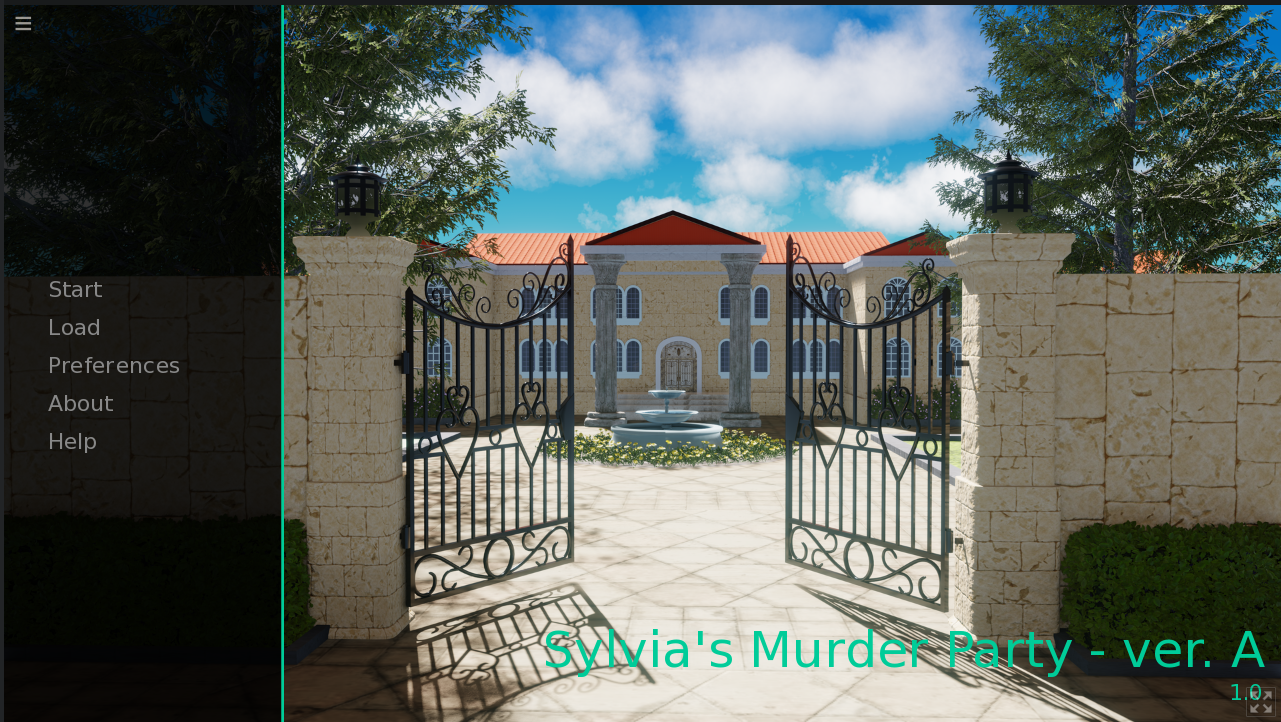
\includegraphics[width=0.9\textwidth]{ch4_1_menu.png}
    \caption{Ekran startowy gry}
    \label{fig:ch4_1_menu}
\end{figure}

\newpage
Przykład prezentacji treści fabularnej jest widoczny na rysunku \ref{fig:ch4_1_intro}. Widok
zasadniczo składa się z tła, opcjonalnie z postaci widocznej na pierwszym planie oraz z panelu
tekstowego (W tym przypadku nie widać imienia postaci więc grający powinien dany fragment uznać
za monolog wewnętrzny głównego bohatera).

\begin{figure}[h!]
    \centering
    
\includegraphics[width=0.9\textwidth]{ch4_1_intro.png}
    \caption{Wprowadzenie fabularne / przykład narracji}
    \label{fig:ch4_1_intro}
\end{figure}

Przykładowy widok dialogu z jedną z postaci NPC został przedstawiony na rysunku \ref{fig:ch4_1_dialogue}.

\begin{figure}[h!]
    \centering
    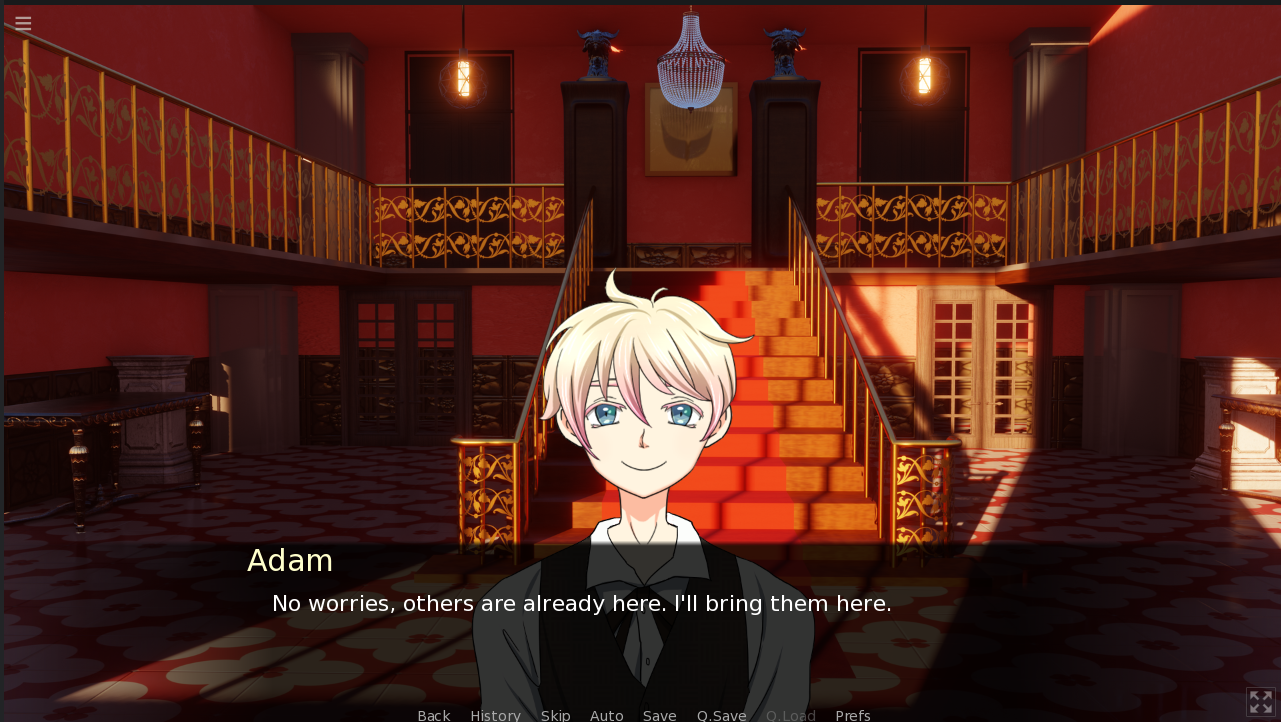
\includegraphics[width=0.9\textwidth]{ch4_1_dialogue.png}
    \caption{Przykładowy dialog z postacią NPC}
    \label{fig:ch4_1_dialogue}
\end{figure}

\subsubsection*{Zarys fabularny}

Gracz zostaje zaproszony na imprezę organizowaną przez Sylvię, bogatą i ekstrawagancką kobietę. Na
przyjęciu pojawiają się również: Adam - marzyciel pracujący w piekarni ojca, Nathaniel -
bezwzględny biznesmen, Randy - genialny pianista o ciemnej stronie, Mary - zmagająca się z
problemami finansowymi pisarka kryminałów oraz Florian - bogaty prawnik zakochany w Sylvii.
Podczas imprezy Sylvia zostaje zamordowana. Gracz znajduje jej ciało i zostawiony list, który
sugeruje jej samobójstwo po czym wzywa policję. Do przyjazdu służb potrzeba kilku godzin, więc
główny bohater postanawia samemu rozwiązać tę sprawę.

Gracz musi rozmawiać z pozostałymi postaciami NPC, zbierając od nich informacje na temat ich
relacji z Sylvią, motywów i alibi w nocy morderstwa. Adam był skrycie zakochany w Sylvii i
zazdrosny o jej związek z Florianem. Nathaniel próbował bezskutecznie przejąć piekarnię ojca Adama.
Randy to utalentowany, ale arogancki pianista z ciemną przeszłością i problemami z prawem,
skrywający wiele tajemnic. Mary to pisarka kryminałów zmagająca się z problemami finansowymi,
będąca najlepszą przyjaciółką Sylvii. Florian to bogaty prawnik zakochany w Sylvii, będący rywalem
Adama w miłości, choć nie zdawał sobie z tego sprawy. Każda postać ma własny charakter i sekrety,
które mogą okazać się istotne dla śledztwa.

Gra kończy się konfrontacją, podczas której gracz wskazuje sprawcę.
W zależności od ostatecznego wyboru może być przedstawione "dobre" lub "złe" zakończenie.

\section{Opis generatywnych agentów}\label{section:ch4_2}

Inworld AI to innowacyjna platforma umożliwiająca tworzenie fotorealistycznych, interaktywnych postaci
wirtualnych, które mogą być wykorzystywane w różnorodnych zastosowaniach. Firma ta oferuje bezkodową
technologię, dzięki której projektowanie postaci staje się niezwykle łatwe i może zostać przeprowadzone w
ciągu zaledwie kilku minut.

Zakres możliwych zastosowań postaci stworzonych za pomocą Inworld AI jest szeroki i obejmuje m.in. gry
wideo otwartego świata, wirtualne awatary i ambasadorów marek, immersyjne doświadczenia edukacyjne oraz
szkolenia. Platforma ta umożliwia tworzenie realistycznie wyglądających i zachowujących się postaci
niezależnych (NPC), które mogą wchodzić w interakcje z użytkownikami w sposób zbliżony do interakcji z
prawdziwymi ludźmi.

W miarę jak przestrzeń sztucznej inteligencji ewoluuje w bardzo szybkim tempie, Inworld AI stale
aktualizuje swoje funkcjonalności, aby optymalizować proces tworzenia postaci i utrzymać pozycję lidera
w dziedzinie generatywnej sztucznej inteligencji. Firma ta kładzie nacisk na ciągłe doskonalenie swoich
technologii, aby zapewnić użytkownikom możliwość tworzenia coraz bardziej realistycznych i zaawansowanych
postaci wirtualnych.

Zastosowanie postaci wygenerowanych przez Inworld AI może przynieść korzyści w wielu branżach, takich
jak rozrywka, marketing, edukacja czy szkolenia. Dzięki ich realistycznemu wyglądowi i zachowaniu, mogą
one zwiększać zaangażowanie użytkowników oraz oferować bardziej immersyjne i angażujące doświadczenia.

\subsubsection*{Kluczowe funkcjonalności platformy Inworld AI}

Wspólna Wiedza (Common Knowledge) umożliwia zdefiniowanie ogólnej wiedzy, która ma być znana przez wiele
postaci. Może to obejmować informacje światobudujące, które wszystkie postacie powinny znać lub wiedzę
przypisaną tylko do konkretnej grupy postaci, np. tych, które wiedzą, że w ich świecie występuje magia
i potrafią jej używać.

Podstawowy Opis (Core Description) stanowi fundament osobowości postaci i w znacznym stopniu wpływa na
wszystkie jej późniejsze reakcje. Powinien koncentrować się na szczegółach dotyczących obecnych
okoliczności życiowych postaci, jej historii, nadziei oraz sposobu w jaki się prezentuje. W tej sekcji
można również wspomnieć o kluczowych relacjach, przedsięwzięciach biznesowych czy lokalizacjach
związanych z daną postacią. Jeśli postać posługuje się specyficzną manierą mówienia lub przestrzega
określonych reguł zachowania, można to tutaj dodać.

W sekcji Motywacje (Motivations) należy umieścić pojedyncze zdania opisujące co motywuje postać do
rozmów z innymi. Może to być chęć realizacji celu lub pragnienia, przedstawienia swojej opinii lub
pomocy użytkownikowi w zdobyciu wiedzy. Ważne jest, aby zastanowić się, co napędza daną postać, ponieważ
będzie to wpływać na jej reakcje, a ona sama będzie poszukiwać okazji do wplatania swoich motywacji w rozmowę.

W polu Wady (Flaws) wpisuje się pojedyncze zdania dotyczące niedoskonałości i lęków postaci. Co
powstrzymuje ją przed realizacją motywacji? W jaki sposób wyraża swoje wewnętrzne konflikty poprzez
zewnętrzny dialog? Jakie tematy wywołają negatywną reakcję?

Rola (Role) zapewnia ramy określające, w jaki sposób postać wchodzi w interakcje z otaczającym ją
światem. Może to być coś ogólnego jak "Bohater" lub "Asystent", ale bardziej szczegółowe archetypy lub
zawody, takie jak "Średniowieczny Wojownik" czy "Ambasador Marki X", lepiej ukierunkują sztuczną
inteligencję Inworld.

Zainteresowania i Hobby (Hobbies and Interests) to krótka lista hobby i zainteresowań postaci. Może
się do nich odwoływać w rozmowie. Mogą być one szerokie (np. pomaganie w rozwiązywaniu problemów
użytkowników) lub specyficzne dla motywacji postaci (np. zasadzanie się na rywalizujące gangi).

Cechy Osobowości (Personality Traits) pomogą stworzyć odpowiednią osobowość i reakcje sztucznej
inteligencji Inworld.

Nastrój i Suwerki Osobowości (Mood and Personality Sliders) decydują o rodzajach emocji, które będzie
przejawiać postać w odpowiedzi na interakcje. Wpływają również na ton jej wypowiedzi - jeśli stworzymy radosną postać, zazwyczaj będzie odpowiadać w radosny sposób.

Fakty i Wiedza (Facts and Knowledge) pomagają w predefiniowaniu odpowiedzi na pytania użytkowników.
Wiedza Osobista to wszystko co postać wie osobiście, natomiast Wspólna Wiedza to miejsce, gdzie można
dodać szersze informacje np. o epoce lub świecie gry, które mogą być współdzielone między wieloma
postaciami. Filtry Wiedzy (Knowledge Filters) mają na celu redukcję odstępstw i niespójności, które
mogłyby wykraczać poza ustalone parametry postaci. Oferowane są trzy poziomy filtrów: Ścisły,
Łagodny i Brak Filtra.

Sekcja Cele (Goals) umożliwia ustawienie specyficznych wyzwalaczy, które spowodują, że postać
zareaguje w określony sposób w konkretnych scenariuszach i interakcjach. Cel działa jako "mechanizm
konsekwencji", który jest aktywowany przez zdarzenie wyzwalające i inicjuje określoną akcję. Pozwala
to twórcom na lepszą kontrolę nad postaciami w czasie rzeczywistym. Dodatkowo, system celów
monitoruje ich osiąganie, wysyłając wyraźny sygnał do klienta po zakończeniu celu.

Styl Dialogu (Dialogue Style) umożliwia wybór spośród szeregu predefiniowanych stylów lub stworzenie
własnego, niestandardowego stylu. Ta funkcja, w połączeniu z Osobowością i Emocjami, zdecyduje o
sposobie, w jaki postać będzie prezentować swoje odpowiedzi. Może być ciekawa i zadawać mnóstwo pytań
lub być tajemnicza i niewiele zdradzać.

Mutacje Postaci (Character Mutations) mają na celu wprowadzanie tymczasowych zmian w atrybutach
postaci, dając więcej kontroli nad nią. Funkcja ta umożliwia implementację postaci przechodzących
przemijające zmiany. Mutacje są częścią systemu celów i pozwalają na modyfikację aktualnie aktywnej
postaci jako akcję celu.

Sceny (Scenes) dostarczają kontekstu, opisując bezpośrednie otoczenie postaci. Jeśli planujemy po
prostu rozmawiać z postacią w studio Inworld lub w Inworld Arcade, nie będziemy musieli dodawać
sceny, chyba że jest to potrzebne dla dodatkowego kontekstu.

\subsubsection*{Opis wykreowanych postaci}

\textbf{Adam} jest marzycielem z małego miasteczka, który pracuje w piekarni swojego ojca. Marzy o lepszym
życiu i pragnie wyrwać się z ciasnych ram swojej codzienności. Zna Floriana z liceum i był
potajemnie zakochany w Sylvii. Czuł zazdrość wobec Floriana z powodu jego relacji z Sylvią.
Adam nienawidzi Nathaniela, który chce wykupić piekarnię jego ojca. Nie przepada również za
Randym, którego uważa za aroganta. W nocy, gdy doszło do morderstwa, był przebudzony, obserwując
Sylvię, i to on znalazł jej ciało.

\textbf{Florian} pochodzi z bogatej rodziny prawniczej. Choć miał wszystko, brakowało mu prawdziwej miłości,
którą znalazł dopiero w Sylvii. Jest osobą lojalną i gotową do poświęceń dla bliskich. Przyjaźnił
się z Adamem od czasów liceum, choć nie wiedział o jego uczuciach do Sylvii. Wiedział, że Sylvia
była najlepszą przyjaciółką Mary. Florian nie lubi Nathaniela za jego metody działania, ale
podziwia talent Randy'ego, nie wiedząc o jego problemach z prawem. Twierdzi, że spał przez całą
noc i nie widział Sylvii przed jej śmiercią.

\textbf{Mary} jest pisarką powieści kryminalnych, która zmaga się z finansowymi problemami. Jej najlepszą
przyjaciółką była Sylvia, która zawsze ją wspierała. Znała Sylvię bardzo dobrze, wiedziała o jej
depresji i problemach. Była w dobrych stosunkach z Nathaniel'em, który próbował pomóc jej w
znalezieniu wydawcy. Mary nie ufa Randy'emu i uważa go za podejrzanego. Gdy doszło do morderstwa,
była w łazience i usłyszała krzyk, ale nie widziała, kto zabił Sylvię.

\textbf{Nathaniel} jest biznesmenem, który dorobił się majątku dzięki swojej determinacji i bezwzględności.
Pragnie zdobyć szacunek, którego nigdy nie zaznał. Podobał mu się Adam, choć ich relacja była
napięta z powodu interesów. Nathaniel cenił Randy'ego za jego talent i wierzył, że po odbyciu kary
więzienia, Randy stał się lepszą osobą. Myślał, że Mary mogłaby zabić z desperacji. Twierdzi, że
spędził noc w kuchni, widząc Randy'ego palącego papierosy na zewnątrz.

\textbf{Randy} to utalentowany pianista z trudną przeszłością. Choć jest podziwiany za swój talent, jego
charakter pozostawia wiele do życzenia – jest arogancki i porywczy. Uważał, że Adam jest podejrzany
z powodu jego zachowania względem Sylvii. Miał mieszane uczucia co do Floriana, którego uważał za
podejrzanego. Wierzył, że Mary potrzebuje prawdziwej inspiracji do swojej pracy. Twierdził, że
spędził noc na zewnątrz, paląc papierosy. W rzeczywistości to on zabił Sylvię, choć stara się to
ukryć.

\subsubsection*{Wykorzystanie agentów w praktyce}

lorfloefleofe

\section{Zaplanowany przebieg eksperymentu}\label{section:ch4_3}

pofkepfokawpefkwpeofk

\subsubsection*{Forma eksperymentu}

lorfloefleofe

\subsubsection*{Gromadzone dane}

lorfloefleofe